%  Grundlagen L-System: Allgemein, Theoretischer Hintergrund, 2D, 3D
\section{L-System}\label{sec:L-System}
Eine zentrale Eigenschaft in der Natur ist die Selbstähnlichkeit von Strukturen auf makroskopischer und mikroskopischer Ebene~\cite{Shaker2016}.
Das heißt, es lassen sich dieselben geometrischen Strukturen in verschiedenen Größenordnungen wiederfinden.
Beispielsweise ähneln die Knospen eines Blumenkohls auch seiner äußeren Struktur, wie in Abbildung~\ref{fig:Blumenkohl}\footnote{Quelle: \url{https://commons.wikimedia.org/wiki/File:Blumenkohl-1.jpg}, Autor: Rainer Zenz, CC BY-SA 3.0 \url{http://creativecommons.org/licenses/by-sa/3.0/}, via Wikimedia Commons} zu sehen ist.
\begin{figure}[ht]
    \centering
    
\includegraphics[width=0.5\linewidth]{chapters/02_Grundlagen/L_System/Blumenkohl-1.jpg}
    \caption{Blumenkohl}\label{fig:Blumenkohl}
\end{figure}

Um diese Eigenschaften präzise und strukturell darzustellen kann ein Lindenmayer-System (L-System)~\cite{lindenmayer1990} eingesetzt werden.
Die Basis eines L-Systems bildet eine kontextfreie Grammatik $G=(N,T,S,P)$ mit einer Menge von Nicht-Terminalsymbolen $N$, einer Menge von Terminalsymbolen $T$, einem Startsymbol $S$ und einer Menge von Produktionen $P$.
Der Unterschied zwischen einem L-System und einer üblichen kontextfreien Grammatik besteht darin, dass in einem Ableitungsschritt eines L-Systems parallel alle Nicht-Terminale ersetzt werden.
Zusätzlich werden nur eine feste Anzahl an Ableitungsschritten durchgeführt und es kann anstatt eines Startsymbols auch ein Startstring angegeben werden.

\subsection{Grafische Darstellung in 2D}
Der resultierende String einer Ableitung kann grafisch als Zeichenvorschriften für \emph{turtle graphics} interpretiert werden.
In \emph{turtle graphics} gibt es eine \emph{turtle}, oder Zeichenkopf, der initial in eine Richtung zeigt und sich in zwei oder drei Dimensionen fortbewegen kann.
Bei jeder Fortbewegung wird entlang der aktuellen Richtung der turtle und der hinterlegten Distanz, eine Strecke gezeichnet.
Die Symbole der Grammatik werden hierbei als Fortbewegung um eine gewisse Distanz oder eine Drehung interpretiert.
In Abbildung~\ref{fig:L-System 2D Rotation} ist eine Visualisierung dieses Konzeptes zu sehen.
Hier ist die turtle initial nach oben gerichtet.

\begin{figure}[ht]
    \centering
    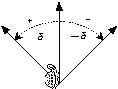
\includegraphics[width=0.5\linewidth]{chapters/02_Grundlagen/L_System/L_System_2D.pdf}
    \caption{L-System 2D Rotation}\label{fig:L-System 2D Rotation}
\end{figure}

Ohne Erweiterungen entstehen hierbei immer zusammenhängende Strukturen, die an einem Stück gezeichnet werden müssen; die turtle darf also nicht springen.
Das heißt, Blätter, Äste oder Stängel sind nur schwer zu realisieren.


\subsection{Erweiterungen}
Um komplexere Strukturen abzubilden, werden zusätzliche Symbole eingesetzt und die Auswertung erweitert.
Zwei übliche Erweiterung, die besonders zur Generierung von Vegetation nützlich sind, sind \emph{Bracketed L-Systeme} und \emph{Stochastische L-Systeme}.

\subsubsection{Bracketed L-Systeme}
\emph{Bracketed L-Systeme}~\cite*{Shaker2016} werden zur Definition von Strukturen eingesetzt, bei denen die turtle ihre Position ändern muss, ohne dass ein Strich gezeichnet wird.
Damit die generierte Struktur zusammenhängend bleibt, wird die Position und aktuelle Richtung der turtle auf einem Stack gespeichert und kann durch \texttt{push} und \texttt{pop} Operationen verwaltet werden.
Die turtle kann sich nur fortbewegen ohne zu zeichnen, indem sie an eine vorherige Position zurückspringt.
Die Menge der Terminalsymbole wird dabei um \texttt{[} für die \texttt{push} Operation und \texttt{]} für \texttt{pop} erweitert.
Bei dem Lesen eines \texttt{[}, wird die aktuelle Position und Rotation der turtle auf dem Stack gespeichert.
Wenn ein \texttt{]} gelesen wird, dann wird die turtle zu der Position und Rotation zurückgesetzt, die auf dem Stack als oberstes Element gespeichert worden war.

Mit dieser Erweiterung können insbesondere auch Äste von Bäumen oder Stängel von Blumen gezeichnet werden.
Ein Beispiel für eine Art von Strauch kann mittels dieses L-Systems erzeugt werden:
\begin{itemize}
    \item Nicht-Terminalsymbole $N=\{F\}$
    \item Terminalsymbole $T=\{\texttt{+},\texttt{-},\texttt{[},\texttt{]}\}$
    \item Startstring $S=F$
    \item Produktionen:
          \begin{align*}
              F\rightarrow~F\texttt{[+}F\texttt{]}F\texttt{[-}F\texttt{]}\texttt{[}F\texttt{]}
          \end{align*}
\end{itemize}

Hierbei beschreibt das Nicht-Terminalsymbol $F$ eine Fortbewegung, \texttt{+} und \texttt{-} jeweils eine Drehung um \ang{30} nach links bzw. rechts in 2D und \texttt{[}, \texttt{]} beschreiben die \texttt{push} und \texttt{pop} Operationen.
Für die ersten drei Ableitungsschritte sind die generierten Strukturen in Abbildung~\ref{fig:Bracketed} dargestellt.

\begin{figure}[ht]
    \begin{subfigure}[t]{.3\textwidth}
        \centering
        \resizebox{!}{100px}{\begin{tikzpicture}\draw (0,0) -- (0,0);
\draw (0,0) -- (0,10);
\draw (0,10) -- (-5,19);
\draw (0,10) -- (0,10);
\draw (0,10) -- (0,20);
\draw (0,20) -- (5,29);
\draw (0,20) -- (0,20);
\draw (0,20) -- (0,30);
\draw (0,20) -- (0,20);
\end{tikzpicture}}

        \caption*{Ein Ableitungsschritt}
    \end{subfigure}
    \hfill
    \begin{subfigure}[t]{.3\textwidth}
        \centering
        \resizebox{!}{100bp}{\begin{tikzpicture}\draw (0,0) -- (0,0);
\draw (0,0) -- (0,10);
\draw (0,10) -- (-5,19);
\draw (0,10) -- (0,10);
\draw (0,10) -- (0,20);
\draw (0,20) -- (5,29);
\draw (0,20) -- (0,20);
\draw (0,20) -- (0,30);
\draw (0,20) -- (0,20);
\draw (0,20) -- (-5,29);
\draw (-5,29) -- (-14,34);
\draw (-5,29) -- (-5,29);
\draw (-5,29) -- (-10,38);
\draw (-10,38) -- (-10,48);
\draw (-10,38) -- (-10,38);
\draw (-10,38) -- (-15,47);
\draw (-10,38) -- (-10,38);
\draw (0,20) -- (0,20);
\draw (0,20) -- (0,30);
\draw (0,30) -- (-5,39);
\draw (0,30) -- (0,30);
\draw (0,30) -- (0,40);
\draw (0,40) -- (5,49);
\draw (0,40) -- (0,40);
\draw (0,40) -- (0,50);
\draw (0,40) -- (0,40);
\draw (0,40) -- (5,49);
\draw (5,49) -- (5,59);
\draw (5,49) -- (5,49);
\draw (5,49) -- (10,58);
\draw (10,58) -- (19,63);
\draw (10,58) -- (10,58);
\draw (10,58) -- (15,67);
\draw (10,58) -- (10,58);
\draw (0,40) -- (0,40);
\draw (0,40) -- (0,50);
\draw (0,50) -- (-5,59);
\draw (0,50) -- (0,50);
\draw (0,50) -- (0,60);
\draw (0,60) -- (5,69);
\draw (0,60) -- (0,60);
\draw (0,60) -- (0,70);
\draw (0,60) -- (0,60);
\draw (0,40) -- (0,40);
\end{tikzpicture}}

        \caption*{Zwei Ableitungsschritte}
    \end{subfigure}
    \hfill
    \begin{subfigure}[t]{.3\textwidth}
        \centering
        \resizebox{!}{100px}{\begin{tikzpicture}\draw (0,0) -- (0,0);
\draw (0,0) -- (0,10);
\draw (0,10) -- (-5,19);
\draw (0,10) -- (0,10);
\draw (0,10) -- (0,20);
\draw (0,20) -- (5,29);
\draw (0,20) -- (0,20);
\draw (0,20) -- (0,30);
\draw (0,20) -- (0,20);
\draw (0,20) -- (-5,29);
\draw (-5,29) -- (-14,34);
\draw (-5,29) -- (-5,29);
\draw (-5,29) -- (-10,38);
\draw (-10,38) -- (-10,48);
\draw (-10,38) -- (-10,38);
\draw (-10,38) -- (-15,47);
\draw (-10,38) -- (-10,38);
\draw (0,20) -- (0,20);
\draw (0,20) -- (0,30);
\draw (0,30) -- (-5,39);
\draw (0,30) -- (0,30);
\draw (0,30) -- (0,40);
\draw (0,40) -- (5,49);
\draw (0,40) -- (0,40);
\draw (0,40) -- (0,50);
\draw (0,40) -- (0,40);
\draw (0,40) -- (5,49);
\draw (5,49) -- (5,59);
\draw (5,49) -- (5,49);
\draw (5,49) -- (10,58);
\draw (10,58) -- (19,63);
\draw (10,58) -- (10,58);
\draw (10,58) -- (15,67);
\draw (10,58) -- (10,58);
\draw (0,40) -- (0,40);
\draw (0,40) -- (0,50);
\draw (0,50) -- (-5,59);
\draw (0,50) -- (0,50);
\draw (0,50) -- (0,60);
\draw (0,60) -- (5,69);
\draw (0,60) -- (0,60);
\draw (0,60) -- (0,70);
\draw (0,60) -- (0,60);
\draw (0,40) -- (0,40);
\draw (0,40) -- (-5,49);
\draw (-5,49) -- (-14,54);
\draw (-5,49) -- (-5,49);
\draw (-5,49) -- (-10,58);
\draw (-10,58) -- (-10,68);
\draw (-10,58) -- (-10,58);
\draw (-10,58) -- (-15,67);
\draw (-10,58) -- (-10,58);
\draw (-10,58) -- (-19,63);
\draw (-19,63) -- (-29,63);
\draw (-19,63) -- (-19,63);
\draw (-19,63) -- (-28,68);
\draw (-28,68) -- (-33,77);
\draw (-28,68) -- (-28,68);
\draw (-28,68) -- (-37,73);
\draw (-28,68) -- (-28,68);
\draw (-10,58) -- (-10,58);
\draw (-10,58) -- (-15,67);
\draw (-15,67) -- (-24,72);
\draw (-15,67) -- (-15,67);
\draw (-15,67) -- (-20,76);
\draw (-20,76) -- (-20,86);
\draw (-20,76) -- (-20,76);
\draw (-20,76) -- (-25,85);
\draw (-20,76) -- (-20,76);
\draw (-20,76) -- (-20,86);
\draw (-20,86) -- (-25,95);
\draw (-20,86) -- (-20,86);
\draw (-20,86) -- (-20,96);
\draw (-20,96) -- (-15,105);
\draw (-20,96) -- (-20,96);
\draw (-20,96) -- (-20,106);
\draw (-20,96) -- (-20,96);
\draw (-20,76) -- (-20,76);
\draw (-20,76) -- (-25,85);
\draw (-25,85) -- (-34,90);
\draw (-25,85) -- (-25,85);
\draw (-25,85) -- (-30,94);
\draw (-30,94) -- (-30,104);
\draw (-30,94) -- (-30,94);
\draw (-30,94) -- (-35,103);
\draw (-30,94) -- (-30,94);
\draw (-20,76) -- (-20,76);
\draw (0,40) -- (0,40);
\draw (0,40) -- (0,50);
\draw (0,50) -- (-5,59);
\draw (0,50) -- (0,50);
\draw (0,50) -- (0,60);
\draw (0,60) -- (5,69);
\draw (0,60) -- (0,60);
\draw (0,60) -- (0,70);
\draw (0,60) -- (0,60);
\draw (0,60) -- (-5,69);
\draw (-5,69) -- (-14,74);
\draw (-5,69) -- (-5,69);
\draw (-5,69) -- (-10,78);
\draw (-10,78) -- (-10,88);
\draw (-10,78) -- (-10,78);
\draw (-10,78) -- (-15,87);
\draw (-10,78) -- (-10,78);
\draw (0,60) -- (0,60);
\draw (0,60) -- (0,70);
\draw (0,70) -- (-5,79);
\draw (0,70) -- (0,70);
\draw (0,70) -- (0,80);
\draw (0,80) -- (5,89);
\draw (0,80) -- (0,80);
\draw (0,80) -- (0,90);
\draw (0,80) -- (0,80);
\draw (0,80) -- (5,89);
\draw (5,89) -- (5,99);
\draw (5,89) -- (5,89);
\draw (5,89) -- (10,98);
\draw (10,98) -- (19,103);
\draw (10,98) -- (10,98);
\draw (10,98) -- (15,107);
\draw (10,98) -- (10,98);
\draw (0,80) -- (0,80);
\draw (0,80) -- (0,90);
\draw (0,90) -- (-5,99);
\draw (0,90) -- (0,90);
\draw (0,90) -- (0,100);
\draw (0,100) -- (5,109);
\draw (0,100) -- (0,100);
\draw (0,100) -- (0,110);
\draw (0,100) -- (0,100);
\draw (0,80) -- (0,80);
\draw (0,80) -- (5,89);
\draw (5,89) -- (5,99);
\draw (5,89) -- (5,89);
\draw (5,89) -- (10,98);
\draw (10,98) -- (19,103);
\draw (10,98) -- (10,98);
\draw (10,98) -- (15,107);
\draw (10,98) -- (10,98);
\draw (10,98) -- (10,108);
\draw (10,108) -- (5,117);
\draw (10,108) -- (10,108);
\draw (10,108) -- (10,118);
\draw (10,118) -- (15,127);
\draw (10,118) -- (10,118);
\draw (10,118) -- (10,128);
\draw (10,118) -- (10,118);
\draw (10,98) -- (10,98);
\draw (10,98) -- (15,107);
\draw (15,107) -- (15,117);
\draw (15,107) -- (15,107);
\draw (15,107) -- (20,116);
\draw (20,116) -- (29,121);
\draw (20,116) -- (20,116);
\draw (20,116) -- (25,125);
\draw (20,116) -- (20,116);
\draw (20,116) -- (29,121);
\draw (29,121) -- (34,130);
\draw (29,121) -- (29,121);
\draw (29,121) -- (38,126);
\draw (38,126) -- (48,126);
\draw (38,126) -- (38,126);
\draw (38,126) -- (47,131);
\draw (38,126) -- (38,126);
\draw (20,116) -- (20,116);
\draw (20,116) -- (25,125);
\draw (25,125) -- (25,135);
\draw (25,125) -- (25,125);
\draw (25,125) -- (30,134);
\draw (30,134) -- (39,139);
\draw (30,134) -- (30,134);
\draw (30,134) -- (35,143);
\draw (30,134) -- (30,134);
\draw (20,116) -- (20,116);
\draw (0,80) -- (0,80);
\draw (0,80) -- (0,90);
\draw (0,90) -- (-5,99);
\draw (0,90) -- (0,90);
\draw (0,90) -- (0,100);
\draw (0,100) -- (5,109);
\draw (0,100) -- (0,100);
\draw (0,100) -- (0,110);
\draw (0,100) -- (0,100);
\draw (0,100) -- (-5,109);
\draw (-5,109) -- (-14,114);
\draw (-5,109) -- (-5,109);
\draw (-5,109) -- (-10,118);
\draw (-10,118) -- (-10,128);
\draw (-10,118) -- (-10,118);
\draw (-10,118) -- (-15,127);
\draw (-10,118) -- (-10,118);
\draw (0,100) -- (0,100);
\draw (0,100) -- (0,110);
\draw (0,110) -- (-5,119);
\draw (0,110) -- (0,110);
\draw (0,110) -- (0,120);
\draw (0,120) -- (5,129);
\draw (0,120) -- (0,120);
\draw (0,120) -- (0,130);
\draw (0,120) -- (0,120);
\draw (0,120) -- (5,129);
\draw (5,129) -- (5,139);
\draw (5,129) -- (5,129);
\draw (5,129) -- (10,138);
\draw (10,138) -- (19,143);
\draw (10,138) -- (10,138);
\draw (10,138) -- (15,147);
\draw (10,138) -- (10,138);
\draw (0,120) -- (0,120);
\draw (0,120) -- (0,130);
\draw (0,130) -- (-5,139);
\draw (0,130) -- (0,130);
\draw (0,130) -- (0,140);
\draw (0,140) -- (5,149);
\draw (0,140) -- (0,140);
\draw (0,140) -- (0,150);
\draw (0,140) -- (0,140);
\draw (0,120) -- (0,120);
\draw (0,80) -- (0,80);
\end{tikzpicture}}

        \caption*{Drei Ableitungsschritte}
    \end{subfigure}
    \caption{Darstellung der ersten drei Ableitungsschritte eines Bracketed L-Systems}\label{fig:Bracketed}
\end{figure}


\subsubsection{Stochastische L-Systeme}
Eine Eigenschaft von den bisher verwendeten L-Systemen ist, dass die Produktionen deterministisch ausgewertet werden und die resultierenden Strings eindeutig sind.
Um realistische Pflanzen generieren zu können muss jedoch etwas Variation eingeführt werden; es wäre also vorteilhaft, wenn die Produktionen nicht-deterministisch ausgewertet werden.
Dazu kann ein \emph{stochastisches L-System}~\cite*{Shaker2016} verwendet werden.
Hierbei kann es mehrere Produktionen mit gleichen linken Seiten geben.
Jeweils über die Menge von Produktionen mit gleicher linken Seite wird eine Wahrscheinlichkeitsverteilung erstellt.
Das heißt die Auswahl der Ersetzung eines Nicht-Terminalsymbols erfolgt zufällig.

Im Folgenden ist ein Beispiel für ein stochastisches Bracketed L-System gegeben:
\begin{itemize}
    \item Nicht-Terminalsymbole $N=\{F\}$
    \item Terminalsymbole $T=\{\texttt{+},\texttt{-},\texttt{[},\texttt{]}\}$
    \item Startstring $S=F$
    \item Produktionen:
          \begin{align*}
              F\xrightarrow{0.33} & ~F\texttt{[+}F\texttt{]}F\texttt{[-}F\texttt{]} F \\
              F\xrightarrow{0.33} & ~F\texttt{[+}F\texttt{]} F                        \\
              F\xrightarrow{0.34} & ~F\texttt{[-}F\texttt{]} F
          \end{align*}
\end{itemize}

Hier gibt es für das Nicht-Terminal $F$ drei Produktionen, zwei Produktionen werden mit einer Wahrscheinlichkeit von \SI{33}{\percent} gewählt und eine Produktion wird mit \SI{34}{\percent} gewählt.
Drei resultierende Bilder dieses L-Systems sind in Abbildung~\ref{fig:Stochastic} gegeben.
Es ist gut erkennbar wie aus einem L-System deutlich unterschiedliche Strukturen generiert werden können, die jedoch alle ähnliche Grundstrukturen aufweisen.
\begin{figure}[ht]
    \begin{subfigure}[t]{.25\textwidth}
        \centering
        \resizebox{!}{175px}{\begin{tikzpicture}\draw (0,0) -- (0,0);
\draw (0,0) -- (0,10);
\draw (0,10) -- (-5,19);
\draw (0,10) -- (0,10);
\draw (0,10) -- (0,20);
\draw (0,20) -- (5,29);
\draw (5,29) -- (5,39);
\draw (5,29) -- (5,29);
\draw (5,29) -- (10,38);
\draw (0,20) -- (0,20);
\draw (0,20) -- (0,30);
\draw (0,30) -- (-5,39);
\draw (0,30) -- (0,30);
\draw (0,30) -- (0,40);
\draw (0,40) -- (5,49);
\draw (5,49) -- (14,54);
\draw (5,49) -- (5,49);
\draw (5,49) -- (10,58);
\draw (10,58) -- (10,68);
\draw (10,68) -- (5,77);
\draw (10,68) -- (10,68);
\draw (10,68) -- (10,78);
\draw (10,58) -- (10,58);
\draw (10,58) -- (15,67);
\draw (15,67) -- (15,77);
\draw (15,67) -- (15,67);
\draw (15,67) -- (20,76);
\draw (0,40) -- (0,40);
\draw (0,40) -- (0,50);
\draw (0,50) -- (5,59);
\draw (0,50) -- (0,50);
\draw (0,50) -- (0,60);
\draw (0,60) -- (-5,69);
\draw (0,60) -- (0,60);
\draw (0,60) -- (0,70);
\draw (0,70) -- (5,79);
\draw (5,79) -- (5,89);
\draw (5,79) -- (5,79);
\draw (5,79) -- (10,88);
\draw (0,70) -- (0,70);
\draw (0,70) -- (0,80);
\draw (0,80) -- (5,89);
\draw (0,80) -- (0,80);
\draw (0,80) -- (0,90);
\draw (0,90) -- (-5,99);
\draw (0,90) -- (0,90);
\draw (0,90) -- (0,100);
\draw (0,100) -- (-5,109);
\draw (-5,109) -- (-5,119);
\draw (-5,109) -- (-5,109);
\draw (-5,109) -- (-10,118);
\draw (-10,118) -- (-19,123);
\draw (-10,118) -- (-10,118);
\draw (-10,118) -- (-15,127);
\draw (-15,127) -- (-15,137);
\draw (-15,137) -- (-10,146);
\draw (-15,137) -- (-15,137);
\draw (-15,137) -- (-15,147);
\draw (-15,127) -- (-15,127);
\draw (-15,127) -- (-20,136);
\draw (-20,136) -- (-20,146);
\draw (-20,136) -- (-20,136);
\draw (-20,136) -- (-25,145);
\draw (-25,145) -- (-34,150);
\draw (-34,150) -- (-44,150);
\draw (-34,150) -- (-34,150);
\draw (-34,150) -- (-43,155);
\draw (-25,145) -- (-25,145);
\draw (-25,145) -- (-30,154);
\draw (-30,154) -- (-30,164);
\draw (-30,154) -- (-30,154);
\draw (-30,154) -- (-35,163);
\draw (-35,163) -- (-44,168);
\draw (-35,163) -- (-35,163);
\draw (-35,163) -- (-40,172);
\draw (0,100) -- (0,100);
\draw (0,100) -- (0,110);
\draw (0,110) -- (-5,119);
\draw (0,110) -- (0,110);
\draw (0,110) -- (0,120);
\draw (0,120) -- (-5,129);
\draw (-5,129) -- (-5,139);
\draw (-5,129) -- (-5,129);
\draw (-5,129) -- (-10,138);
\draw (-10,138) -- (-19,143);
\draw (-10,138) -- (-10,138);
\draw (-10,138) -- (-15,147);
\draw (0,120) -- (0,120);
\draw (0,120) -- (0,130);
\draw (0,130) -- (5,139);
\draw (0,130) -- (0,130);
\draw (0,130) -- (0,140);
\draw (0,140) -- (-5,149);
\draw (0,140) -- (0,140);
\draw (0,140) -- (0,150);
\draw (0,150) -- (5,159);
\draw (5,159) -- (14,164);
\draw (5,159) -- (5,159);
\draw (5,159) -- (10,168);
\draw (10,168) -- (10,178);
\draw (10,168) -- (10,168);
\draw (10,168) -- (15,177);
\draw (15,177) -- (24,182);
\draw (24,182) -- (29,191);
\draw (24,182) -- (24,182);
\draw (24,182) -- (33,187);
\draw (15,177) -- (15,177);
\draw (15,177) -- (20,186);
\draw (20,186) -- (29,191);
\draw (20,186) -- (20,186);
\draw (20,186) -- (25,195);
\draw (25,195) -- (25,205);
\draw (25,205) -- (30,214);
\draw (25,205) -- (25,205);
\draw (25,205) -- (25,215);
\draw (25,215) -- (20,224);
\draw (25,215) -- (25,215);
\draw (25,215) -- (25,225);
\draw (25,225) -- (30,234);
\draw (30,234) -- (39,239);
\draw (30,234) -- (30,234);
\draw (30,234) -- (35,243);
\draw (35,243) -- (35,253);
\draw (35,243) -- (35,243);
\draw (35,243) -- (40,252);
\draw (25,225) -- (25,225);
\draw (25,225) -- (25,235);
\draw (25,235) -- (20,244);
\draw (25,235) -- (25,235);
\draw (25,235) -- (25,245);
\draw (25,245) -- (20,254);
\draw (20,254) -- (20,264);
\draw (20,254) -- (20,254);
\draw (20,254) -- (15,263);
\draw (25,245) -- (25,245);
\draw (25,245) -- (25,255);
\draw (25,255) -- (30,264);
\draw (25,255) -- (25,255);
\draw (25,255) -- (25,265);
\draw (25,265) -- (20,274);
\draw (25,265) -- (25,265);
\draw (25,265) -- (25,275);
\draw (25,195) -- (25,195);
\draw (25,195) -- (30,204);
\draw (30,204) -- (30,214);
\draw (30,204) -- (30,204);
\draw (30,204) -- (35,213);
\draw (35,213) -- (35,223);
\draw (35,223) -- (30,232);
\draw (35,223) -- (35,223);
\draw (35,223) -- (35,233);
\draw (35,213) -- (35,213);
\draw (35,213) -- (40,222);
\draw (40,222) -- (49,227);
\draw (40,222) -- (40,222);
\draw (40,222) -- (45,231);
\draw (45,231) -- (45,241);
\draw (45,231) -- (45,231);
\draw (45,231) -- (50,240);
\draw (0,150) -- (0,150);
\draw (0,150) -- (0,160);
\draw (0,160) -- (-5,169);
\draw (0,160) -- (0,160);
\draw (0,160) -- (0,170);
\draw (0,170) -- (5,179);
\draw (5,179) -- (14,184);
\draw (5,179) -- (5,179);
\draw (5,179) -- (10,188);
\draw (10,188) -- (10,198);
\draw (10,188) -- (10,188);
\draw (10,188) -- (15,197);
\draw (0,170) -- (0,170);
\draw (0,170) -- (0,180);
\draw (0,180) -- (-5,189);
\draw (0,180) -- (0,180);
\draw (0,180) -- (0,190);
\draw (0,190) -- (5,199);
\draw (5,199) -- (14,204);
\draw (5,199) -- (5,199);
\draw (5,199) -- (10,208);
\draw (10,208) -- (10,218);
\draw (10,208) -- (10,208);
\draw (10,208) -- (15,217);
\draw (15,217) -- (24,222);
\draw (24,222) -- (29,231);
\draw (24,222) -- (24,222);
\draw (24,222) -- (33,227);
\draw (15,217) -- (15,217);
\draw (15,217) -- (20,226);
\draw (20,226) -- (29,231);
\draw (20,226) -- (20,226);
\draw (20,226) -- (25,235);
\draw (25,235) -- (25,245);
\draw (25,245) -- (30,254);
\draw (25,245) -- (25,245);
\draw (25,245) -- (25,255);
\draw (25,235) -- (25,235);
\draw (25,235) -- (30,244);
\draw (30,244) -- (39,249);
\draw (30,244) -- (30,244);
\draw (30,244) -- (35,253);
\draw (0,190) -- (0,190);
\draw (0,190) -- (0,200);
\draw (0,200) -- (5,209);
\draw (0,200) -- (0,200);
\draw (0,200) -- (0,210);
\draw (0,210) -- (-5,219);
\draw (0,210) -- (0,210);
\draw (0,210) -- (0,220);
\draw (0,220) -- (5,229);
\draw (5,229) -- (14,234);
\draw (5,229) -- (5,229);
\draw (5,229) -- (10,238);
\draw (0,220) -- (0,220);
\draw (0,220) -- (0,230);
\draw (0,230) -- (5,239);
\draw (0,230) -- (0,230);
\draw (0,230) -- (0,240);
\draw (0,240) -- (-5,249);
\draw (0,240) -- (0,240);
\draw (0,240) -- (0,250);
\draw (0,250) -- (-5,259);
\draw (-5,259) -- (-14,264);
\draw (-5,259) -- (-5,259);
\draw (-5,259) -- (-10,268);
\draw (-10,268) -- (-19,273);
\draw (-19,273) -- (-24,282);
\draw (-19,273) -- (-19,273);
\draw (-19,273) -- (-28,278);
\draw (-10,268) -- (-10,268);
\draw (-10,268) -- (-15,277);
\draw (-15,277) -- (-15,287);
\draw (-15,277) -- (-15,277);
\draw (-15,277) -- (-20,286);
\draw (-20,286) -- (-29,291);
\draw (-20,286) -- (-20,286);
\draw (-20,286) -- (-25,295);
\draw (-25,295) -- (-25,305);
\draw (-25,305) -- (-20,314);
\draw (-25,305) -- (-25,305);
\draw (-25,305) -- (-25,315);
\draw (-25,315) -- (-30,324);
\draw (-25,315) -- (-25,315);
\draw (-25,315) -- (-25,325);
\draw (-25,325) -- (-30,334);
\draw (-30,334) -- (-30,344);
\draw (-30,334) -- (-30,334);
\draw (-30,334) -- (-35,343);
\draw (-25,325) -- (-25,325);
\draw (-25,325) -- (-25,335);
\draw (-25,335) -- (-30,344);
\draw (-25,335) -- (-25,335);
\draw (-25,335) -- (-25,345);
\draw (-25,295) -- (-25,295);
\draw (-25,295) -- (-30,304);
\draw (-30,304) -- (-30,314);
\draw (-30,304) -- (-30,304);
\draw (-30,304) -- (-35,313);
\draw (-35,313) -- (-44,318);
\draw (-35,313) -- (-35,313);
\draw (-35,313) -- (-40,322);
\draw (-40,322) -- (-40,332);
\draw (-40,332) -- (-35,341);
\draw (-40,332) -- (-40,332);
\draw (-40,332) -- (-40,342);
\draw (-40,322) -- (-40,322);
\draw (-40,322) -- (-45,331);
\draw (-45,331) -- (-45,341);
\draw (-45,331) -- (-45,331);
\draw (-45,331) -- (-50,340);
\draw (-50,340) -- (-59,345);
\draw (-50,340) -- (-50,340);
\draw (-50,340) -- (-55,349);
\draw (-55,349) -- (-64,354);
\draw (-64,354) -- (-69,363);
\draw (-64,354) -- (-64,354);
\draw (-64,354) -- (-73,359);
\draw (-73,359) -- (-83,359);
\draw (-73,359) -- (-73,359);
\draw (-73,359) -- (-82,364);
\draw (-55,349) -- (-55,349);
\draw (-55,349) -- (-60,358);
\draw (-60,358) -- (-69,363);
\draw (-60,358) -- (-60,358);
\draw (-60,358) -- (-65,367);
\draw (0,250) -- (0,250);
\draw (0,250) -- (0,260);
\draw (0,260) -- (5,269);
\draw (0,260) -- (0,260);
\draw (0,260) -- (0,270);
\draw (0,270) -- (-5,279);
\draw (-5,279) -- (-5,289);
\draw (-5,279) -- (-5,279);
\draw (-5,279) -- (-10,288);
\draw (0,270) -- (0,270);
\draw (0,270) -- (0,280);
\draw (0,280) -- (5,289);
\draw (0,280) -- (0,280);
\draw (0,280) -- (0,290);
\draw (0,290) -- (-5,299);
\draw (0,290) -- (0,290);
\draw (0,290) -- (0,300);
\draw (0,300) -- (5,309);
\draw (5,309) -- (5,319);
\draw (5,309) -- (5,309);
\draw (5,309) -- (10,318);
\draw (10,318) -- (19,323);
\draw (19,323) -- (24,332);
\draw (19,323) -- (19,323);
\draw (19,323) -- (28,328);
\draw (10,318) -- (10,318);
\draw (10,318) -- (15,327);
\draw (15,327) -- (15,337);
\draw (15,327) -- (15,327);
\draw (15,327) -- (20,336);
\draw (20,336) -- (20,346);
\draw (20,346) -- (15,355);
\draw (20,346) -- (20,346);
\draw (20,346) -- (20,356);
\draw (20,336) -- (20,336);
\draw (20,336) -- (25,345);
\draw (25,345) -- (34,350);
\draw (25,345) -- (25,345);
\draw (25,345) -- (30,354);
\draw (30,354) -- (30,364);
\draw (30,354) -- (30,354);
\draw (30,354) -- (35,363);
\draw (0,300) -- (0,300);
\draw (0,300) -- (0,310);
\draw (0,310) -- (-5,319);
\draw (0,310) -- (0,310);
\draw (0,310) -- (0,320);
\draw (0,320) -- (5,329);
\draw (5,329) -- (14,334);
\draw (5,329) -- (5,329);
\draw (5,329) -- (10,338);
\draw (10,338) -- (10,348);
\draw (10,338) -- (10,338);
\draw (10,338) -- (15,347);
\draw (0,320) -- (0,320);
\draw (0,320) -- (0,330);
\draw (0,330) -- (5,339);
\draw (0,330) -- (0,330);
\draw (0,330) -- (0,340);
\draw (0,340) -- (-5,349);
\draw (-5,349) -- (-14,354);
\draw (-5,349) -- (-5,349);
\draw (-5,349) -- (-10,358);
\draw (-10,358) -- (-10,368);
\draw (-10,368) -- (-5,377);
\draw (-10,368) -- (-10,368);
\draw (-10,368) -- (-10,378);
\draw (-10,358) -- (-10,358);
\draw (-10,358) -- (-15,367);
\draw (-15,367) -- (-15,377);
\draw (-15,367) -- (-15,367);
\draw (-15,367) -- (-20,376);
\draw (-20,376) -- (-29,381);
\draw (-20,376) -- (-20,376);
\draw (-20,376) -- (-25,385);
\draw (0,340) -- (0,340);
\draw (0,340) -- (0,350);
\draw (0,350) -- (-5,359);
\draw (0,350) -- (0,350);
\draw (0,350) -- (0,360);
\draw (0,360) -- (5,369);
\draw (5,369) -- (14,374);
\draw (5,369) -- (5,369);
\draw (5,369) -- (10,378);
\draw (0,360) -- (0,360);
\draw (0,360) -- (0,370);
\draw (0,370) -- (-5,379);
\draw (0,370) -- (0,370);
\draw (0,370) -- (0,380);
\draw (0,380) -- (-5,389);
\draw (-5,389) -- (-14,394);
\draw (-5,389) -- (-5,389);
\draw (-5,389) -- (-10,398);
\draw (0,380) -- (0,380);
\draw (0,380) -- (0,390);
\draw (0,390) -- (5,399);
\draw (0,390) -- (0,390);
\draw (0,390) -- (0,400);
\draw (0,400) -- (-5,409);
\draw (0,400) -- (0,400);
\draw (0,400) -- (0,410);
\end{tikzpicture}}

    \end{subfigure}
    \hfill
    \begin{subfigure}[t]{.25\textwidth}
        \centering
        \resizebox{!}{175bp}{\begin{tikzpicture}\draw (0,0) -- (0,0);
\draw (0,0) -- (0,10);
\draw (0,10) -- (5,19);
\draw (0,10) -- (0,10);
\draw (0,10) -- (0,20);
\draw (0,20) -- (5,29);
\draw (5,29) -- (5,39);
\draw (5,29) -- (5,29);
\draw (5,29) -- (10,38);
\draw (0,20) -- (0,20);
\draw (0,20) -- (0,30);
\draw (0,30) -- (5,39);
\draw (0,30) -- (0,30);
\draw (0,30) -- (0,40);
\draw (0,40) -- (-5,49);
\draw (0,40) -- (0,40);
\draw (0,40) -- (0,50);
\draw (0,50) -- (-5,59);
\draw (-5,59) -- (-5,69);
\draw (-5,59) -- (-5,59);
\draw (-5,59) -- (-10,68);
\draw (-10,68) -- (-19,73);
\draw (-10,68) -- (-10,68);
\draw (-10,68) -- (-15,77);
\draw (0,50) -- (0,50);
\draw (0,50) -- (0,60);
\draw (0,60) -- (5,69);
\draw (0,60) -- (0,60);
\draw (0,60) -- (0,70);
\draw (0,70) -- (-5,79);
\draw (-5,79) -- (-14,84);
\draw (-5,79) -- (-5,79);
\draw (-5,79) -- (-10,88);
\draw (-10,88) -- (-10,98);
\draw (-10,98) -- (-15,107);
\draw (-10,98) -- (-10,98);
\draw (-10,98) -- (-10,108);
\draw (-10,88) -- (-10,88);
\draw (-10,88) -- (-15,97);
\draw (-15,97) -- (-24,102);
\draw (-15,97) -- (-15,97);
\draw (-15,97) -- (-20,106);
\draw (-20,106) -- (-29,111);
\draw (-29,111) -- (-39,111);
\draw (-29,111) -- (-29,111);
\draw (-29,111) -- (-38,116);
\draw (-20,106) -- (-20,106);
\draw (-20,106) -- (-25,115);
\draw (-25,115) -- (-34,120);
\draw (-25,115) -- (-25,115);
\draw (-25,115) -- (-30,124);
\draw (0,70) -- (0,70);
\draw (0,70) -- (0,80);
\draw (0,80) -- (5,89);
\draw (0,80) -- (0,80);
\draw (0,80) -- (0,90);
\draw (0,90) -- (-5,99);
\draw (0,90) -- (0,90);
\draw (0,90) -- (0,100);
\draw (0,100) -- (5,109);
\draw (5,109) -- (5,119);
\draw (5,109) -- (5,109);
\draw (5,109) -- (10,118);
\draw (0,100) -- (0,100);
\draw (0,100) -- (0,110);
\draw (0,110) -- (-5,119);
\draw (0,110) -- (0,110);
\draw (0,110) -- (0,120);
\draw (0,120) -- (-5,129);
\draw (-5,129) -- (-5,139);
\draw (-5,129) -- (-5,129);
\draw (-5,129) -- (-10,138);
\draw (-10,138) -- (-19,143);
\draw (-10,138) -- (-10,138);
\draw (-10,138) -- (-15,147);
\draw (-15,147) -- (-15,157);
\draw (-15,157) -- (-10,166);
\draw (-15,157) -- (-15,157);
\draw (-15,157) -- (-15,167);
\draw (-15,147) -- (-15,147);
\draw (-15,147) -- (-20,156);
\draw (-20,156) -- (-20,166);
\draw (-20,156) -- (-20,156);
\draw (-20,156) -- (-25,165);
\draw (-25,165) -- (-34,170);
\draw (-25,165) -- (-25,165);
\draw (-25,165) -- (-30,174);
\draw (-30,174) -- (-30,184);
\draw (-30,184) -- (-25,193);
\draw (-30,184) -- (-30,184);
\draw (-30,184) -- (-30,194);
\draw (-30,194) -- (-25,203);
\draw (-25,203) -- (-25,213);
\draw (-25,203) -- (-25,203);
\draw (-25,203) -- (-20,212);
\draw (-30,194) -- (-30,194);
\draw (-30,194) -- (-30,204);
\draw (-30,204) -- (-25,213);
\draw (-30,204) -- (-30,204);
\draw (-30,204) -- (-30,214);
\draw (-30,214) -- (-35,223);
\draw (-35,223) -- (-35,233);
\draw (-35,223) -- (-35,223);
\draw (-35,223) -- (-40,232);
\draw (-40,232) -- (-49,237);
\draw (-40,232) -- (-40,232);
\draw (-40,232) -- (-45,241);
\draw (-30,214) -- (-30,214);
\draw (-30,214) -- (-30,224);
\draw (-30,224) -- (-25,233);
\draw (-30,224) -- (-30,224);
\draw (-30,224) -- (-30,234);
\draw (-30,234) -- (-35,243);
\draw (-30,234) -- (-30,234);
\draw (-30,234) -- (-30,244);
\draw (-30,174) -- (-30,174);
\draw (-30,174) -- (-35,183);
\draw (-35,183) -- (-35,193);
\draw (-35,183) -- (-35,183);
\draw (-35,183) -- (-40,192);
\draw (-40,192) -- (-49,197);
\draw (-40,192) -- (-40,192);
\draw (-40,192) -- (-45,201);
\draw (-45,201) -- (-54,206);
\draw (-54,206) -- (-64,206);
\draw (-54,206) -- (-54,206);
\draw (-54,206) -- (-63,211);
\draw (-45,201) -- (-45,201);
\draw (-45,201) -- (-50,210);
\draw (-50,210) -- (-50,220);
\draw (-50,210) -- (-50,210);
\draw (-50,210) -- (-55,219);
\draw (-55,219) -- (-64,224);
\draw (-55,219) -- (-55,219);
\draw (-55,219) -- (-60,228);
\draw (-60,228) -- (-69,233);
\draw (-69,233) -- (-79,233);
\draw (-69,233) -- (-69,233);
\draw (-69,233) -- (-78,238);
\draw (-78,238) -- (-83,247);
\draw (-83,247) -- (-83,257);
\draw (-83,247) -- (-83,247);
\draw (-83,247) -- (-88,256);
\draw (-78,238) -- (-78,238);
\draw (-78,238) -- (-87,243);
\draw (-87,243) -- (-97,243);
\draw (-87,243) -- (-87,243);
\draw (-87,243) -- (-96,248);
\draw (-60,228) -- (-60,228);
\draw (-60,228) -- (-65,237);
\draw (-65,237) -- (-74,242);
\draw (-65,237) -- (-65,237);
\draw (-65,237) -- (-70,246);
\draw (-70,246) -- (-70,256);
\draw (-70,256) -- (-65,265);
\draw (-70,256) -- (-70,256);
\draw (-70,256) -- (-70,266);
\draw (-70,246) -- (-70,246);
\draw (-70,246) -- (-75,255);
\draw (-75,255) -- (-84,260);
\draw (-75,255) -- (-75,255);
\draw (-75,255) -- (-80,264);
\draw (-80,264) -- (-89,269);
\draw (-89,269) -- (-94,278);
\draw (-89,269) -- (-89,269);
\draw (-89,269) -- (-98,274);
\draw (-98,274) -- (-108,274);
\draw (-98,274) -- (-98,274);
\draw (-98,274) -- (-107,279);
\draw (-80,264) -- (-80,264);
\draw (-80,264) -- (-85,273);
\draw (-85,273) -- (-85,283);
\draw (-85,273) -- (-85,273);
\draw (-85,273) -- (-90,282);
\draw (-90,282) -- (-99,287);
\draw (-90,282) -- (-90,282);
\draw (-90,282) -- (-95,291);
\draw (0,120) -- (0,120);
\draw (0,120) -- (0,130);
\draw (0,130) -- (5,139);
\draw (0,130) -- (0,130);
\draw (0,130) -- (0,140);
\draw (0,140) -- (-5,149);
\draw (0,140) -- (0,140);
\draw (0,140) -- (0,150);
\draw (0,150) -- (-5,159);
\draw (-5,159) -- (-14,164);
\draw (-5,159) -- (-5,159);
\draw (-5,159) -- (-10,168);
\draw (0,150) -- (0,150);
\draw (0,150) -- (0,160);
\draw (0,160) -- (5,169);
\draw (0,160) -- (0,160);
\draw (0,160) -- (0,170);
\draw (0,170) -- (-5,179);
\draw (-5,179) -- (-5,189);
\draw (-5,179) -- (-5,179);
\draw (-5,179) -- (-10,188);
\draw (-10,188) -- (-19,193);
\draw (-10,188) -- (-10,188);
\draw (-10,188) -- (-15,197);
\draw (-15,197) -- (-15,207);
\draw (-15,207) -- (-20,216);
\draw (-15,207) -- (-15,207);
\draw (-15,207) -- (-15,217);
\draw (-15,197) -- (-15,197);
\draw (-15,197) -- (-20,206);
\draw (-20,206) -- (-29,211);
\draw (-20,206) -- (-20,206);
\draw (-20,206) -- (-25,215);
\draw (0,170) -- (0,170);
\draw (0,170) -- (0,180);
\draw (0,180) -- (-5,189);
\draw (0,180) -- (0,180);
\draw (0,180) -- (0,190);
\draw (0,190) -- (-5,199);
\draw (-5,199) -- (-5,209);
\draw (-5,199) -- (-5,199);
\draw (-5,199) -- (-10,208);
\draw (0,190) -- (0,190);
\draw (0,190) -- (0,200);
\draw (0,200) -- (5,209);
\draw (0,200) -- (0,200);
\draw (0,200) -- (0,210);
\draw (0,210) -- (-5,219);
\draw (0,210) -- (0,210);
\draw (0,210) -- (0,220);
\end{tikzpicture}}

    \end{subfigure}
    \hfill
    \begin{subfigure}[t]{.25\textwidth}
        \centering
        \resizebox{!}{175px}{\begin{tikzpicture}\draw (0,0) -- (0,0);
\draw (0,0) -- (0,10);
\draw (0,10) -- (5,19);
\draw (0,10) -- (0,10);
\draw (0,10) -- (0,20);
\draw (0,20) -- (-5,29);
\draw (0,20) -- (0,20);
\draw (0,20) -- (0,30);
\draw (0,30) -- (-5,39);
\draw (-5,39) -- (-14,44);
\draw (-5,39) -- (-5,39);
\draw (-5,39) -- (-10,48);
\draw (0,30) -- (0,30);
\draw (0,30) -- (0,40);
\draw (0,40) -- (-5,49);
\draw (0,40) -- (0,40);
\draw (0,40) -- (0,50);
\draw (0,50) -- (-5,59);
\draw (-5,59) -- (-5,69);
\draw (-5,59) -- (-5,59);
\draw (-5,59) -- (-10,68);
\draw (-10,68) -- (-19,73);
\draw (-19,73) -- (-29,73);
\draw (-19,73) -- (-19,73);
\draw (-19,73) -- (-28,78);
\draw (-10,68) -- (-10,68);
\draw (-10,68) -- (-15,77);
\draw (-15,77) -- (-15,87);
\draw (-15,77) -- (-15,77);
\draw (-15,77) -- (-20,86);
\draw (-20,86) -- (-29,91);
\draw (-20,86) -- (-20,86);
\draw (-20,86) -- (-25,95);
\draw (0,50) -- (0,50);
\draw (0,50) -- (0,60);
\draw (0,60) -- (5,69);
\draw (0,60) -- (0,60);
\draw (0,60) -- (0,70);
\draw (0,70) -- (-5,79);
\draw (0,70) -- (0,70);
\draw (0,70) -- (0,80);
\draw (0,80) -- (5,89);
\draw (5,89) -- (14,94);
\draw (5,89) -- (5,89);
\draw (5,89) -- (10,98);
\draw (0,80) -- (0,80);
\draw (0,80) -- (0,90);
\draw (0,90) -- (-5,99);
\draw (0,90) -- (0,90);
\draw (0,90) -- (0,100);
\draw (0,100) -- (-5,109);
\draw (-5,109) -- (-5,119);
\draw (-5,109) -- (-5,109);
\draw (-5,109) -- (-10,118);
\draw (0,100) -- (0,100);
\draw (0,100) -- (0,110);
\draw (0,110) -- (5,119);
\draw (0,110) -- (0,110);
\draw (0,110) -- (0,120);
\draw (0,120) -- (-5,129);
\draw (0,120) -- (0,120);
\draw (0,120) -- (0,130);
\draw (0,130) -- (5,139);
\draw (5,139) -- (5,149);
\draw (5,139) -- (5,139);
\draw (5,139) -- (10,148);
\draw (10,148) -- (19,153);
\draw (19,153) -- (24,162);
\draw (19,153) -- (19,153);
\draw (19,153) -- (28,158);
\draw (10,148) -- (10,148);
\draw (10,148) -- (15,157);
\draw (15,157) -- (24,162);
\draw (15,157) -- (15,157);
\draw (15,157) -- (20,166);
\draw (20,166) -- (20,176);
\draw (20,166) -- (20,166);
\draw (20,166) -- (25,175);
\draw (25,175) -- (34,180);
\draw (34,180) -- (44,180);
\draw (34,180) -- (34,180);
\draw (34,180) -- (43,185);
\draw (43,185) -- (48,194);
\draw (43,185) -- (43,185);
\draw (43,185) -- (52,190);
\draw (52,190) -- (57,199);
\draw (57,199) -- (66,204);
\draw (57,199) -- (57,199);
\draw (57,199) -- (62,208);
\draw (62,208) -- (62,218);
\draw (62,208) -- (62,208);
\draw (62,208) -- (67,217);
\draw (52,190) -- (52,190);
\draw (52,190) -- (61,195);
\draw (61,195) -- (66,204);
\draw (61,195) -- (61,195);
\draw (61,195) -- (70,200);
\draw (25,175) -- (25,175);
\draw (25,175) -- (30,184);
\draw (30,184) -- (30,194);
\draw (30,184) -- (30,184);
\draw (30,184) -- (35,193);
\draw (35,193) -- (35,203);
\draw (35,203) -- (40,212);
\draw (35,203) -- (35,203);
\draw (35,203) -- (35,213);
\draw (35,193) -- (35,193);
\draw (35,193) -- (40,202);
\draw (40,202) -- (40,212);
\draw (40,202) -- (40,202);
\draw (40,202) -- (45,211);
\draw (0,130) -- (0,130);
\draw (0,130) -- (0,140);
\draw (0,140) -- (5,149);
\draw (0,140) -- (0,140);
\draw (0,140) -- (0,150);
\draw (0,150) -- (-5,159);
\draw (-5,159) -- (-5,169);
\draw (-5,159) -- (-5,159);
\draw (-5,159) -- (-10,168);
\draw (-10,168) -- (-19,173);
\draw (-10,168) -- (-10,168);
\draw (-10,168) -- (-15,177);
\draw (0,150) -- (0,150);
\draw (0,150) -- (0,160);
\draw (0,160) -- (-5,169);
\draw (0,160) -- (0,160);
\draw (0,160) -- (0,170);
\draw (0,170) -- (5,179);
\draw (5,179) -- (5,189);
\draw (5,179) -- (5,179);
\draw (5,179) -- (10,188);
\draw (10,188) -- (19,193);
\draw (19,193) -- (29,193);
\draw (19,193) -- (19,193);
\draw (19,193) -- (28,198);
\draw (28,198) -- (33,207);
\draw (28,198) -- (28,198);
\draw (28,198) -- (37,203);
\draw (10,188) -- (10,188);
\draw (10,188) -- (15,197);
\draw (15,197) -- (24,202);
\draw (15,197) -- (15,197);
\draw (15,197) -- (20,206);
\draw (20,206) -- (20,216);
\draw (20,206) -- (20,206);
\draw (20,206) -- (25,215);
\draw (25,215) -- (25,225);
\draw (25,225) -- (20,234);
\draw (25,225) -- (25,225);
\draw (25,225) -- (25,235);
\draw (25,215) -- (25,215);
\draw (25,215) -- (30,224);
\draw (30,224) -- (39,229);
\draw (30,224) -- (30,224);
\draw (30,224) -- (35,233);
\draw (0,170) -- (0,170);
\draw (0,170) -- (0,180);
\draw (0,180) -- (5,189);
\draw (0,180) -- (0,180);
\draw (0,180) -- (0,190);
\draw (0,190) -- (5,199);
\draw (5,199) -- (14,204);
\draw (5,199) -- (5,199);
\draw (5,199) -- (10,208);
\draw (10,208) -- (10,218);
\draw (10,208) -- (10,208);
\draw (10,208) -- (15,217);
\draw (0,190) -- (0,190);
\draw (0,190) -- (0,200);
\draw (0,200) -- (5,209);
\draw (0,200) -- (0,200);
\draw (0,200) -- (0,210);
\draw (0,210) -- (-5,219);
\draw (-5,219) -- (-5,229);
\draw (-5,219) -- (-5,219);
\draw (-5,219) -- (-10,228);
\draw (-10,228) -- (-19,233);
\draw (-10,228) -- (-10,228);
\draw (-10,228) -- (-15,237);
\draw (-15,237) -- (-15,247);
\draw (-15,247) -- (-10,256);
\draw (-15,247) -- (-15,247);
\draw (-15,247) -- (-15,257);
\draw (-15,237) -- (-15,237);
\draw (-15,237) -- (-20,246);
\draw (-20,246) -- (-20,256);
\draw (-20,246) -- (-20,246);
\draw (-20,246) -- (-25,255);
\draw (-25,255) -- (-34,260);
\draw (-34,260) -- (-44,260);
\draw (-34,260) -- (-34,260);
\draw (-34,260) -- (-43,265);
\draw (-25,255) -- (-25,255);
\draw (-25,255) -- (-30,264);
\draw (-30,264) -- (-39,269);
\draw (-30,264) -- (-30,264);
\draw (-30,264) -- (-35,273);
\draw (-35,273) -- (-44,278);
\draw (-44,278) -- (-49,287);
\draw (-44,278) -- (-44,278);
\draw (-44,278) -- (-53,283);
\draw (-53,283) -- (-63,283);
\draw (-53,283) -- (-53,283);
\draw (-53,283) -- (-62,288);
\draw (-62,288) -- (-67,297);
\draw (-67,297) -- (-76,302);
\draw (-67,297) -- (-67,297);
\draw (-67,297) -- (-72,306);
\draw (-62,288) -- (-62,288);
\draw (-62,288) -- (-71,293);
\draw (-71,293) -- (-76,302);
\draw (-71,293) -- (-71,293);
\draw (-71,293) -- (-80,298);
\draw (-80,298) -- (-90,298);
\draw (-80,298) -- (-80,298);
\draw (-80,298) -- (-89,303);
\draw (-35,273) -- (-35,273);
\draw (-35,273) -- (-40,282);
\draw (-40,282) -- (-40,292);
\draw (-40,282) -- (-40,282);
\draw (-40,282) -- (-45,291);
\draw (-45,291) -- (-45,301);
\draw (-45,301) -- (-40,310);
\draw (-45,301) -- (-45,301);
\draw (-45,301) -- (-45,311);
\draw (-45,311) -- (-50,320);
\draw (-45,311) -- (-45,311);
\draw (-45,311) -- (-45,321);
\draw (-45,291) -- (-45,291);
\draw (-45,291) -- (-50,300);
\draw (-50,300) -- (-59,305);
\draw (-50,300) -- (-50,300);
\draw (-50,300) -- (-55,309);
\draw (-55,309) -- (-64,314);
\draw (-64,314) -- (-69,323);
\draw (-64,314) -- (-64,314);
\draw (-64,314) -- (-73,319);
\draw (-55,309) -- (-55,309);
\draw (-55,309) -- (-60,318);
\draw (-60,318) -- (-60,328);
\draw (-60,318) -- (-60,318);
\draw (-60,318) -- (-65,327);
\draw (0,210) -- (0,210);
\draw (0,210) -- (0,220);
\draw (0,220) -- (5,229);
\draw (0,220) -- (0,220);
\draw (0,220) -- (0,230);
\draw (0,230) -- (-5,239);
\draw (-5,239) -- (-5,249);
\draw (-5,239) -- (-5,239);
\draw (-5,239) -- (-10,248);
\draw (-10,248) -- (-19,253);
\draw (-10,248) -- (-10,248);
\draw (-10,248) -- (-15,257);
\draw (0,230) -- (0,230);
\draw (0,230) -- (0,240);
\draw (0,240) -- (5,249);
\draw (0,240) -- (0,240);
\draw (0,240) -- (0,250);
\draw (0,250) -- (-5,259);
\draw (0,250) -- (0,250);
\draw (0,250) -- (0,260);
\draw (0,260) -- (-5,269);
\draw (-5,269) -- (-5,279);
\draw (-5,269) -- (-5,269);
\draw (-5,269) -- (-10,278);
\draw (-10,278) -- (-10,288);
\draw (-10,288) -- (-5,297);
\draw (-10,288) -- (-10,288);
\draw (-10,288) -- (-10,298);
\draw (-10,278) -- (-10,278);
\draw (-10,278) -- (-15,287);
\draw (-15,287) -- (-15,297);
\draw (-15,287) -- (-15,287);
\draw (-15,287) -- (-20,296);
\draw (-20,296) -- (-29,301);
\draw (-29,301) -- (-39,301);
\draw (-29,301) -- (-29,301);
\draw (-29,301) -- (-38,306);
\draw (-20,296) -- (-20,296);
\draw (-20,296) -- (-25,305);
\draw (-25,305) -- (-25,315);
\draw (-25,305) -- (-25,305);
\draw (-25,305) -- (-30,314);
\draw (-30,314) -- (-39,319);
\draw (-30,314) -- (-30,314);
\draw (-30,314) -- (-35,323);
\draw (0,260) -- (0,260);
\draw (0,260) -- (0,270);
\draw (0,270) -- (-5,279);
\draw (0,270) -- (0,270);
\draw (0,270) -- (0,280);
\draw (0,280) -- (5,289);
\draw (5,289) -- (14,294);
\draw (5,289) -- (5,289);
\draw (5,289) -- (10,298);
\draw (0,280) -- (0,280);
\draw (0,280) -- (0,290);
\draw (0,290) -- (5,299);
\draw (0,290) -- (0,290);
\draw (0,290) -- (0,300);
\end{tikzpicture}}

    \end{subfigure}
    \caption{Drei Resultate desselben stochastischen L-Systems}\label{fig:Stochastic}
\end{figure}


\subsubsection{Erweiterung in 3D}\label{subsub: L-System 3D}
Die L-Systeme aus den vorherigen Abschnitten haben stets zweidimensionale Strukturen erstellt.
Dabei wurden die Symbole \texttt{+} und \texttt{-} genutzt um die aktuelle Richtung der turtle in der Ebene zu rotieren.
Für Strukturen in drei Dimensionen kann diese Idee weiterverwendet werden.
Hierbei werden jeweils zwei Symbole für Rotationen um jede der drei Achsen eingeführt.
Die Symbole \texttt{+} und \texttt{-} rotieren die turtle um die $z$-Achse, \texttt{\&} und \texttt{\textasciicircum} rotieren um die $x$-Achse und \texttt{/} und \texttt{\textbackslash} rotieren um die $y$-Achse.

Ein Beispiel\footnote{L-System adaptiert von: \url{https://www.sidefx.com/docs/houdini/nodes/sop/lsystem.html\#3d}} für ein L-System, das einen dreidimensionalen Baum erzeugt ist im Folgenden gegeben:
\begin{itemize}
    \item Nicht-Terminalsymbole $N=\{F\}$
    \item Terminalsymbole $T=\{\texttt{+},\texttt{-},\texttt{\&},\texttt{\textasciicircum},\texttt{/},\texttt{\textbackslash},\texttt{[},\texttt{]}\}$
    \item Startstring $S=FFFA$
    \item Produktionen:
          \begin{align*}
              A\rightarrow & ~\texttt{[}B\texttt{]////[}B\texttt{]////}B \\
              B\rightarrow & ~\texttt{\&}FFFA
          \end{align*}
\end{itemize}

Mit diesem L-System kann ein dreidimensionaler Baum wie in Abbildung~\ref{fig:L-System 3D Unity} in Unity erzeugt werden.
Es wurden 7 Ableitungsschritte durchgeführt und es wurde jeweils \ang{28} um die Achsen rotiert.

\begin{figure}[ht]
    \centering
    % \resizebox{\linewidth-3cm}{!}{%
    
    % }
    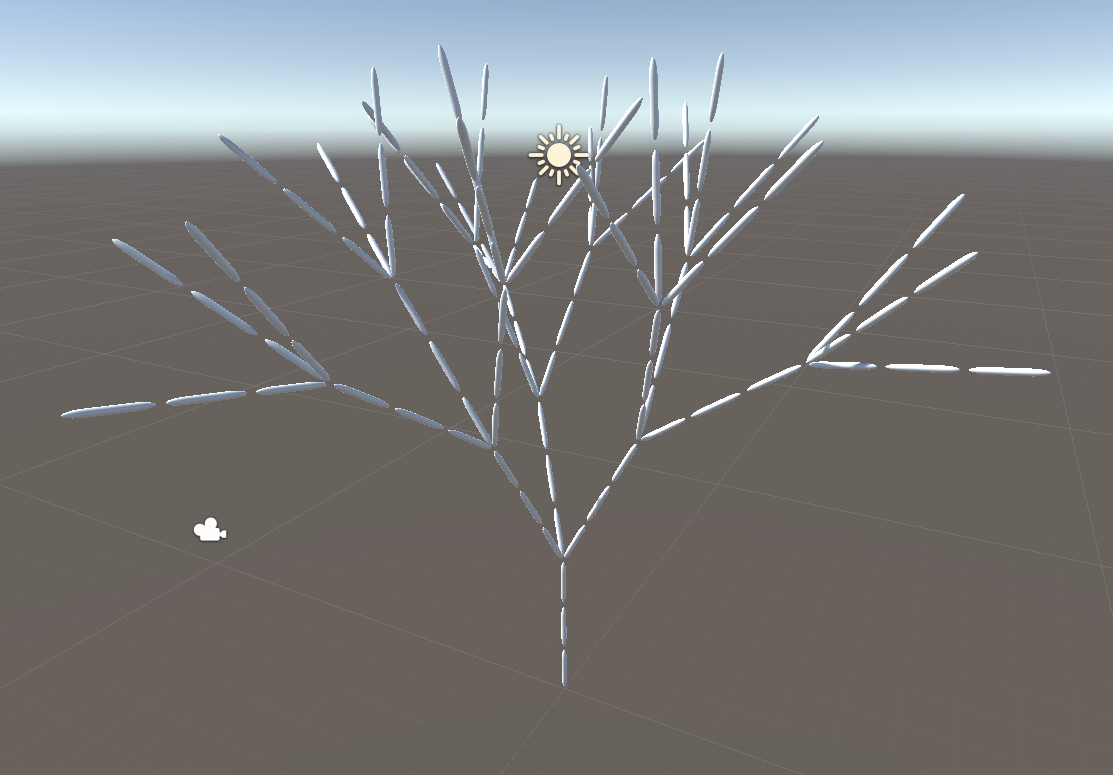
\includegraphics[width=0.5\linewidth]{chapters/02_Grundlagen/L_System/L_System_3D_Tree.png}
    \caption{L-System 3D Baum}\label{fig:L-System 3D Unity}
\end{figure}


\subsection{Auswertung eines L-Systems}
Die Auswertung eines L-Systems wird in diesem Abschnitt beschrieben.
Der Algorithmus~\ref{alg:L-System Auswertung} umfasst die, ausgehend vom Startstring, durchgeführten $i$ Ableitungsschritte der Grammatik.
Der Startstring wird Zeichen-für-Zeichen von links nach rechts durchlaufen und es wird für jede Iteration ein leerer String als Zwischenresultat angelegt.
Für jedes gelesene Zeichen des Startstrings wird überprüft, ob es sich um ein Nicht-Terminalsymbol oder Terminalsymbol handelt.
Im Falle eines Nicht-Terminalsymbols wird die Ersetzung gemäß der entsprechenden Produktion an das Zwischenresultat angehangen.
Ein Terminalsymbol wird einfach in das Zwischenresultat übernommen.
In jeder Iteration wird der Startstring vollständig durchlaufen.
Dadurch werden alle Nicht-Terminale des Startstrings der jeweiligen Iteration ersetzt.
Am Ende der $n$-ten Iteration wird das Zwischenresultat als neuen Startstring für die $n+1$-te Iteration gesetzt und der Prozess wiederholt sich für die festgelegten $i$ Iterationen.
Für ein stochastisches L-System muss die Wahl der Ersetzung in Zeile 6 gemäß der Wahrscheinlichkeiten für das Nicht-Terminalsymbol erfolgen.

\begin{algorithm}[H]
    \begin{algorithmic}[1]
        \footnotesize
        \REQUIRE{Grammatik $(N,T,S,P)$, Iterationen $i$}
        \ENSURE{String $w$ nach $i$ Ableitungsschritten}
        \STATE{$w \gets S$}
        \FOR{$i$ Iterationen}
        \STATE{$temp\gets \emptyset$}
        \FOR{$c\in w$}
        \IF{$c\in N$}
        \STATE{Wähle Ersetzung $r$ aus Produktion mit $(c\rightarrow r)\in P$}
        \STATE{Hänge $r$ an $temp$ an}
        \ELSE
        \STATE{Hänge $c$ an $temp$ an}
        \ENDIF
        \ENDFOR
        \STATE{$w\gets temp$}
        \ENDFOR
        \RETURN{$w$}
    \end{algorithmic}
    \caption{L-System Auswertung}\label{alg:L-System Auswertung}
\end{algorithm}
